% !TeX spellcheck = fr_FR

\chapter{Chapitre 4 : Résultats}
Dans ce chapitre, nous allons voir les résultats obtenus par les
différentes parties de l'application. On va aussi comparer les différentes
métriques collectées des binaires.

Les tests suivants ont été réalisés principalement sur la configuration d'ordinateur
se trouvant dans la figure \ref{fig:computer_configuration} en annexe 4.

\section{Triangulation}

La triangulation de Delaunay provient en grande partie du projet de semestre.
Seule la partie fusion de maillage a été implémentée dans ce travail.

Pour la triangulation, on utilise deux fichiers:
\begin{itemize}
	\item Le fichier 2501500\_1112000.las du jeu de données des \gls{sitg} contenant 9'000'987 points
	\item Un fichier contenant que les 100'000 premiers points du fichier précédent.
\end{itemize}

\subsection{Algorithme de Bowyer-Watson}

\begin{table}[htbp!]
	\begin{tabular}{l|c|c|c|c|}
		\cline{2-5}
		\multicolumn{1}{c|}{}                              & Nb Points                    & \begin{tabular}[c]{@{}c@{}}Temps moyen\\ {[}s{]}\end{tabular} & Nb Trig                     & \begin{tabular}[c]{@{}c@{}}Taille de sortie\\ {[}Mb{]}\end{tabular} \\ \hline
		\multicolumn{1}{|l|}{2501500\_1112000\_sample.las} & \multicolumn{1}{l|}{100'000} & \multicolumn{1}{c|}{6,646}                              & \multicolumn{1}{l|}{199928} & 9.6 Mb                                                              \\ \hline
		\multicolumn{1}{|l|}{2501500\_1112000.las}         & 9'000'987                    & N/A                                                           & N/A                         & N/A                                                                 \\ \hline
	\end{tabular}
	\caption{Résultats de la triangulation avec l'algorithme Bowyer-Watson}
	\label{tab:triangulation_results}
\end{table}

Dans le tableau \ref{tab:triangulation_results}, on peut observer que sur un
fichier de plusieurs millions de points aucune valeur n'est présente. L'implémentation actuelle n'arrivant pas à
exécuter en un temps raisonnable, les valeurs ici manquent.

\subsection{Algorithme Delaunator}

Cette partie utilise une implémentation de la triangulation de Delaunay
existante. Il s'agit de l'algorithme delaunator implémentant des idées de S-hull
et de sweepline triangulation.

Les résultats suivants montrent l'efficacité de cette implémentation par rapport à
l'implémentation de Bowyer-Watson.

\begin{table}[htbp!]
	\begin{tabular}{l|c|c|c|c|}
		\cline{2-5}
		\multicolumn{1}{c|}{}                              & Nb Points                    & \begin{tabular}[c]{@{}c@{}}Temps moyen\\ {[}s{]}\end{tabular} & Nb Trig                      & \begin{tabular}[c]{@{}c@{}}Taille de sortie\\ {[}Mb{]}\end{tabular} \\ \hline
		\multicolumn{1}{|l|}{2501500\_1112000\_sample.las} & \multicolumn{1}{l|}{100'000} & \multicolumn{1}{c|}{0,0513}                             & \multicolumn{1}{c|}{199'928} & 9.6                                                                 \\ \hline
		\multicolumn{1}{|l|}{2501500\_1112000.las}         & 9'000'987                    & 9,548                                                   & 18'001'310                   & 859                                                                 \\ \hline
	\end{tabular}
	\caption{Résultats de la triangulation avec l'algorithme delaunator}
	\label{tab:triangulation_delaunator_result}
\end{table}

\subsection{Fusion de triangulation}

Les résultats de la fusion ne sont pas disponibles, car le binaire actuel ne
soumet pas de fichiers de sortie.

On peut observer le flamegraph de la figure \ref{fig:flamegraph_mesh_merge}
du binaire ou le programme reste bloqué dans la méthode \textit{get\_side\_candidate}
avant que ce dernier soit interrompu.

\begin{figure}[htbp!]
    \centering
    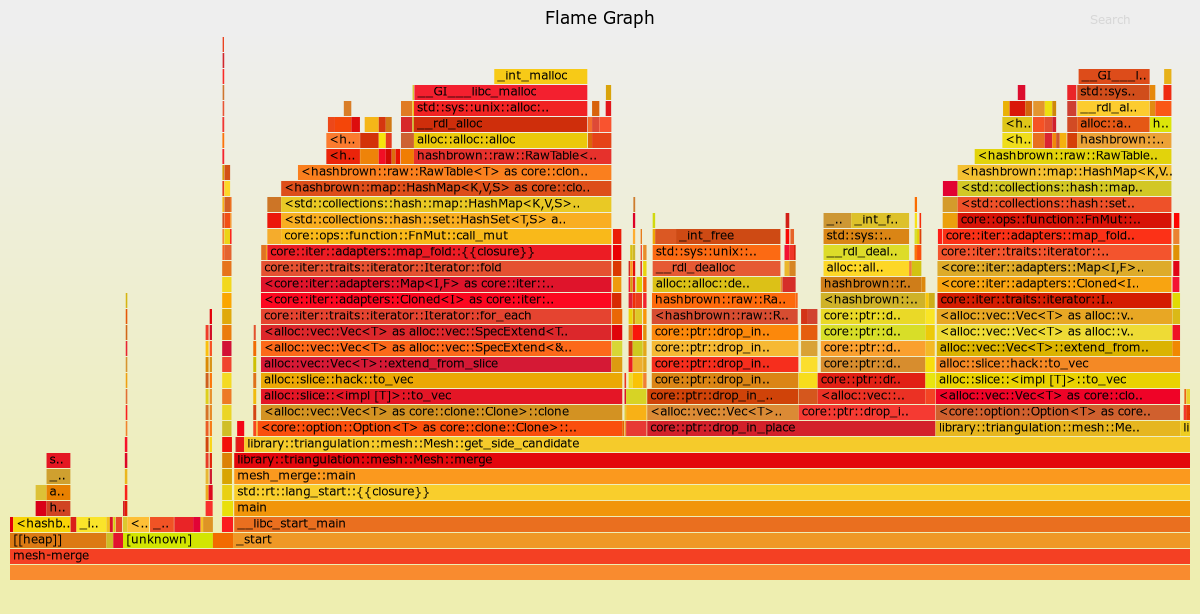
\includegraphics[width=0.8\linewidth]{figures/merge-debug-flamegraph.png}
    \caption{Flamegraph du binaire mesh-merge. Source : réalisé par Jérôme Chételat}
    \label{fig:flamegraph_mesh_merge}
\end{figure}


Cependant les tests unitaires valident l'algorithme pour un jeu de données simple.

\textbf{Améliorations possibles}

L'implémentation actuelle gère uniquement les maillages linéairement séparables.
L'idée serait de pouvoir aussi gérer le cas ou les maillages peuvent se
superposer.

On a aussi le problème que l'algorithme ne s'applique que dans une direction
pour créer des arrêtés. Le principe serait d'implémenter un choix de direction
pour appliquer la fusion.

\section{Nettoyage}

Le nettoyage de points est effectué sur deux fichiers lidars:
\begin{enumerate}
    \item 2488500\_1111500.las
    \item 2499000\_1118000.las
\end{enumerate}

Pour les maillages on effectue les tests sur deux fichiers \gls{stl}, résultant des triangulations des fichiers précédent.

\subsection{Lidar}
Voici les résultats obtenus:

\textbf{Point moyen}

\begin{table}[htb!]
\begin{tabular}{l|c|c|c|c|c|}
\cline{2-6}
\multicolumn{1}{c|}{}                      & Nb Points & Temps  & Points supprimés & Taille originale & Taille de sortie \\ \hline
\multicolumn{1}{|l|}{2488500\_1111500.las} & 8'570'137 & 4.67 s & 1'147'625        & 229 Mo          & 199 Mo           \\ \hline
\multicolumn{1}{|l|}{2499000\_1118000.las} & 9'336'496 & 4.96 s & 1'000'136        & 250 Mo          & 223 Mo           \\ \hline
\end{tabular}
\caption{Résultats du nettoyage par point moyen}
\label{tab:las_cleaning_avg}
\end{table}

\textbf{Point pondéré}

\begin{table}[htb!]
\begin{tabular}{l|c|c|c|c|c|}
\cline{2-6}
\multicolumn{1}{c|}{}                      & Nb Points & Temps  & Points supprimés & Taille originale & Taille de sortie \\ \hline
\multicolumn{1}{|l|}{2488500\_1111500.las} & 8'570'137 & 4.87 s & 1'147'625        & 229 Mo          & 199 Mo           \\ \hline
\multicolumn{1}{|l|}{2499000\_1118000.las} & 9'336'496 & 5.03 s & 1'000'136        & 250 Mo          & 223 Mo           \\ \hline
\end{tabular}
\caption{Résultats du nettoyage par point pondéré}
\label{tab:las_cleaning_ponderated}
\end{table}

On observe aucune différence de taille de sortie ni de nombre de points supprimés entre les deux méthodes.
Cela s'explique par le choix de la méthode de nettoyage.
Ici le nombre d'impulsions à retour multiple reste constant et donc le nombre de points à supprimer ne varie pas.

Cependant, on observe des différences de position des points lidars dans les figures de l'annexe 5.

\subsection{Lissage de maillage}

Le lissage a été effectué avec un epsilon de 2.0.
Voici les résultats obtenus sur un maillage comportant une route: 

\begin{figure}[htbp!]
    \centering
    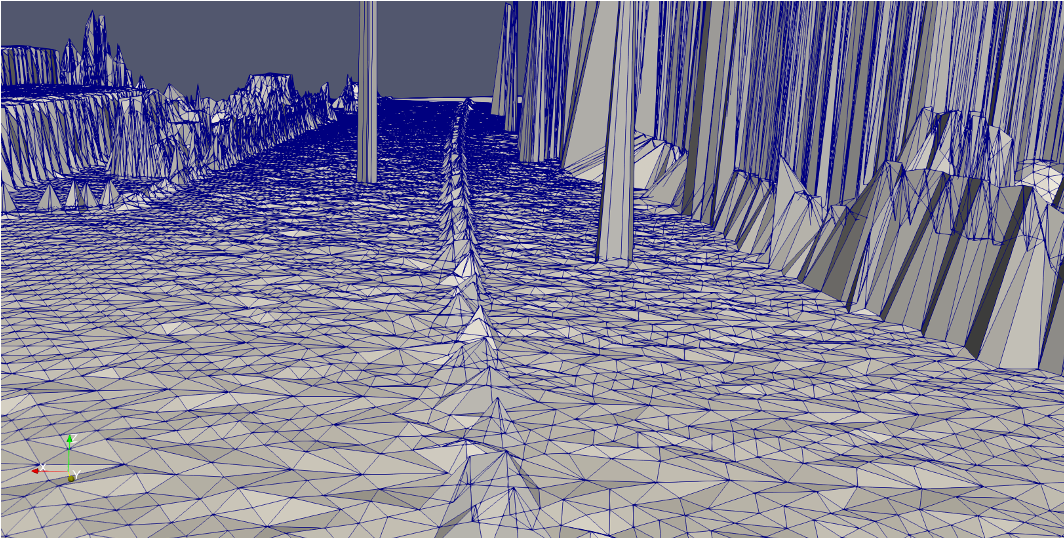
\includegraphics[width=0.8\linewidth]{figures/mesh_noise.png}
    \caption{Maillage bruité avec une route avant lissage. Source : réalisé par Jérôme Chételat}
    \label{fig:mesh_noise}
\end{figure}

\begin{figure}[htbp!]
    \centering
    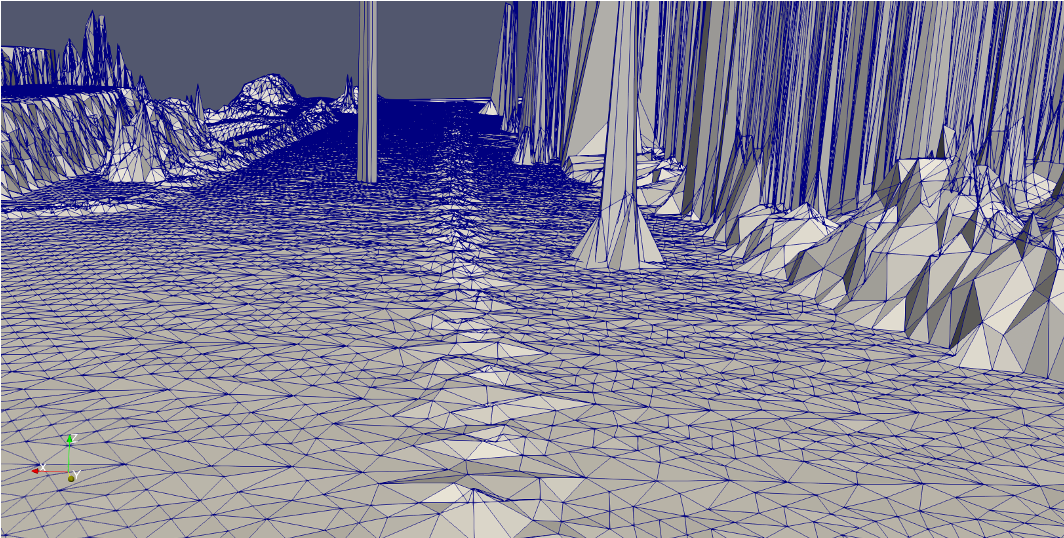
\includegraphics[width=0.8\linewidth]{figures/mesh_noise_not_noise.png}
    \caption{Maillage avec une route après lissage. Source : réalisé par Jérôme Chételat}
    \label{fig:mesh_noise_not_noise}
\end{figure}

\begin{figure}[htbp!]
    \centering
    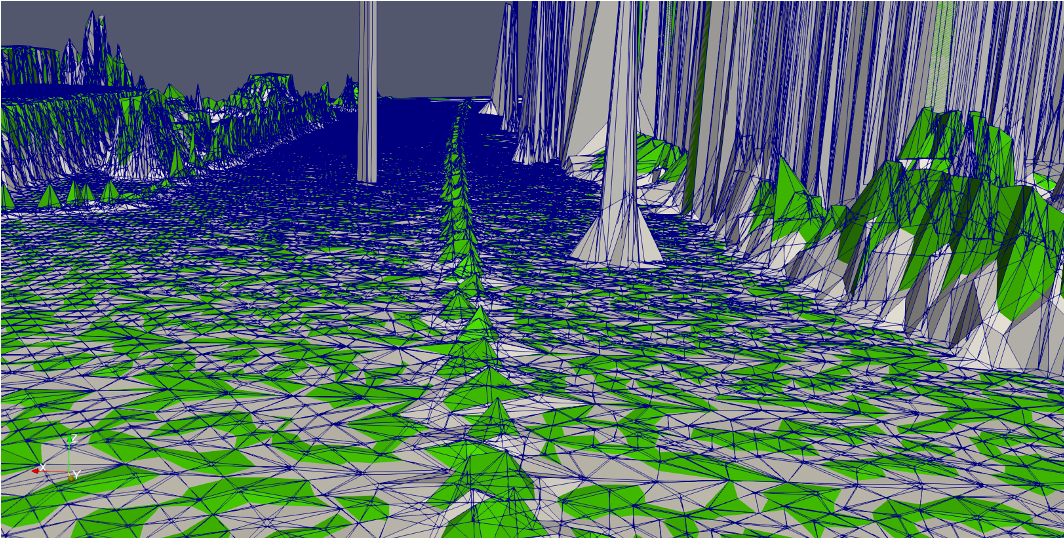
\includegraphics[width=0.8\linewidth]{figures/mesh_noise_difference.png}
    \caption{Différence d'élévation des maillages après lissage. Vert: maillage de base. Source : réalisé par Jérôme Chételat}
    \label{fig:mesh_noise_diff}
\end{figure}

On observe dans les images précédentes que le lissage rend les surfaces planes et que les pics ne perdent pas d'élévation au-dessus d'un certain $\epsilon$.

\subsection{Décimation de maillage}

\section{Stack Web}
\subsection{Serveur web}

Le serveur actuel permet le téléchargement de fichiers \gls{stl} présents dans
un dossier spécifique. Il arrive à servir des fichiers avec les mécaniques \gls{cors}.

\subsection{Client web}
Les tests suivants ont été effectués sur le navigateur Firefox version 80.0.1.
Le client web permet actuellement de faire un rendu d'un maillage dans un
navigateur web. Un fichier \gls{stl} est téléchargé à l'aide de l'api
\textit{fetch} du navigateur au chargement de la page web.

On peut observer dans la figure \ref{fig:web_client} en annexe 6 qu'une grande partie de la page est blanche.
Ce phénomène est normal, car le rendu se fait sans ombres.
De ce fait, cela rend l'observation des changements d'élévation des surfaces difficile.
Cependant, on peut voir que le contour de la partie blanche laisse imaginer qu'il y a bien un rendu de maillage présent.

On y observe aussi que dans un tableau de \textit{Float32} se trouve 300'000 valeurs qui correspondent aux 100'000 sommets du maillage (une valeur par composante de la position d'un point).

\textbf{Améliorations possibles} \\
Le chargement des vertex du maillage se faisant dans un seul file d'exécution,
la page lors du chargement reste figée et peut ne plus répondre (dépend de la
puissance de l'hôte) .
Il serait possible dans un futur proche de faire ces opérations dans des WebWorkers. Au
moment de l'écriture de ce mémoire, l'utilisation des WebWorkers
en Rust est encore expérimentale.

Une autre amélioration à faire serait de réaliser le calcul des ombres afin d'afficher les reliefs du maillage.
Ou encore de donner des contrôles à l'utilisateur pour changer le point 
de vue du maillage (angle et position de la caméra dans la scène).
